\section{Onderzoeksonderwerpen}
Voor het onderzoeksrapport moeten opties worden onderzocht voor de meest geschikte manier van implementatie van het project. Op te beginnen moet er worden bestudeerd hoe het huidige systeem precies werkt. Tevens moet er worden uitgezocht welke frameworks er als beste kunnen worden gebruikt. Er moet een framework voor het datatransport worden uitgezocht en een framework voor de GUI. Daarnaast moet ook worden gekeken op welke manier de data van het exoskelet naar de externe bron gaat worden verzonden. Hiervoor moet zowel naar hardware als software worden gekeken.
\subsection{Hoe werkt het huidige systeem}
In het huidige systeem wordt met behulp van Simulink alle gegevens uit de sensoren verzameld. Hoe dit precies werkt en of het relevant is moet nog worden uitgezocht. 
\subsection{Model}
Voor het model is het huidige idee om de data van het exoskelet naar een receiver te sturen. Deze schoont dan de data op, en stuurt de data door naar mogelijk meerdere instanties van de interface.
\begin{figure}[!ht]
	\centering
	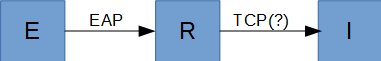
\includegraphics[width=150px]{ERIModel}
	\caption{Schematische weergave van het model. \textit{E} staat voor het exoskelet, \textit{R} staat voor de receiver en \textit{I} staat voor de interface.}
\end{figure}
\subsection{Frameworks}
\subsubsection{GUI}
Voor de GUI is een framework nodig wat 3D-visualisatie ondersteunt.
\subsubsection{Dataverbinding naar GUI}
Er is een framework nodig dat de data die binnenkomt in Simulink omzet in data die kan worden gebruikt door de GUI. Hierbij moet rekening worden gehouden met het feit dat MatLab een beperkt aantal programmeertalen ondersteunt.
\subsection{Connectiviteitsopties}
\subsubsection{Hardware}
Er is momenteel nog geen hardware beschikbaar om een verbinding te maken tussen het exoskelet en de receiver. Het exoskelet heeft zowel een USB-poort als een Ethernet-poort, wat de opties voor mogelijke hardware redelijk uitgebreid maakt.
\subsubsection{Software}
Het beoogde protocol om de data te verzenden is momenteel het EtherCAT Automation Protocol (EAP). Naar verwachting heeft EAP alle benodigde functionaliteiten.